\documentclass[12pt]{article}

\usepackage[utf8]{inputenc}
\usepackage[danish]{babel}
\usepackage{latexsym, amsfonts, amssymb, amsthm, amsmath, siunitx, graphicx, pgfplots}
\usepackage[hidelinks]{hyperref}

\sisetup{exponent-product = \cdot,
  output-decimal-marker = {,}}

%Giles Castelles incfig
\usepackage{import}
\usepackage{xifthen}
\usepackage{pdfpages}
\usepackage{transparent}

\newcommand{\incfig}[2][1]{%
  \def\svgwidth{#1\columnwidth}
  \import{../figures/}{#2.pdf_tex}
}

\pdfsuppresswarningpagegroup=1

\setlength{\parindent}{0in}
\setlength{\oddsidemargin}{0in}
\setlength{\textwidth}{6.5in}
\setlength{\textheight}{8.8in}
\setlength{\topmargin}{0in}
\setlength{\headheight}{18pt}

\pgfplotsset{compat=newest}

\pgfplotsset{every axis/.append style={
  axis x line=middle,    % put the x axis in the middle
  axis y line=middle,    % put the y axis in the middle
  axis line style={<->,color=black}, % arrows on the axis
}}

\title{Opgaver til forelæsning 12}
\author{Noah Rahbek Bigum Hansen}
\date{15. Oktober 2024}

\begin{document}

\maketitle

\section*{Opg. 8.47}
Blocks $A$ (mass \qty{2,00}{kg}) and $B$ (mass \qty{6,00}{kg}) move on a frictionless, horizontal surface. Initially, block $B$ is at rest and block $A$ is moving toward it at \qty{2,00}{m/s}. The blocks are equipped with ideal spring bumpers, as in Example 8.10 (Section 8.4). The collision is head-on, so all motion before and after the collision is along a straight line.

\subsection*{(a)}
Find the maximum energy stored in the spring bumpers and the velocity of each block at that time.
\bigbreak
Fra konservation af impuls har vi at
\[
m_a\cdot v_{ax_1} + 0 = (m_a + m_b)v_{2x} \implies v_{2x} = \frac{m_a\cdot v_{ax_1}}{m_a+m_b}
.\] 
Den kinetiske energi før \textit{impacten} er
\[
k_1 = \frac{1}{2} \cdot m_a \cdot \left( v_{ax_1} \right)^2  
.\] 
Og efter \textit{impacten} er den kinetiske energi
\[
k_2 = \frac{1}{2} \cdot (m_a + m_b) \cdot \left( v_{x_2} \right)^2  \implies k_2 = \frac{1}{2}(m_a + m_b) \cdot \left( \frac{m_a}{m_a + m_b} \right)^2 v_{ax_{1}}^2
.\]
Energien gemt i fjedrene når de er trykket helt sammen bliver da differensen mellem den kinetiske energi før impacten. Altså har vi at
\[
U_s = k_1 - k_2 = \frac{1}{2} \cdot m_a \cdot \left( v_{ax_1} \right)^2 - \frac{1}{2}(m_a + m_b) \cdot \left( \frac{m_a}{m_a+m_b} \right) ^2 v_{ax_1}^2 \implies U_s = \frac{m_a m_b}{2(m_a + m_b)}v_{ax_1}^2 
.\]
Der indsættes kendte værdier
\[
U_s = \frac{\qty{2,00}{kg}\cdot \qty{6,00}{kg}}{2\left( \qty{2,00}{kg} + \qty{6,00}{kg} \right)} \left( \qty{2,00}{\frac{m}{s}} \right)^2 = \qty{3,00}{J}
.\] 

\subsection*{(b)}
Find the velocity of each block after they have moved apart.
\bigbreak
Vi har fra konservation af impuls at
\[
m_a + v_{ax_1} = m_a \cdot  v_{ax_2} + m_b \cdot v_{bx_2} 
.\] 
Derudover er kinetisk energi konserveret
\[
k = \frac{1}{2} \cdot m_a \cdot \left( v_{ax_1} \right)^2 = \frac{1}{2} \cdot m_a \cdot \left( v_{ax_2} \right)^2 + \frac{1}{2} \cdot m_b \cdot \left( v_{bx_2} \right)^2  
.\]
Dermed har vi at
\[
v_{ax_2} = \frac{m_a-m_b}{m_a + m_b}v_{ax_1} \implies v_{ax_2} = \frac{\qty{2,00}{kg} - \qty{6,00}{kg}}{\qty{2,00}{kg} + \qty{6,00}{kg}} \cdot \qty{2,00}{\frac{m}{s}} = \qty{-1,00}{\frac{m}{s}}
.\]
Og
\[
v_{bx_2} = \frac{2m_a}{m_a+m_b} = \frac{2\cdot \qty{2,00}{kg}}{\qty{2,00}{kg} + \qty{6,00}{kg}}\cdot \qty{2,00}{\frac{m}{s}} = \qty{1,00}{\frac{m}{s}}
.\] 


\section*{Opg. 8.53}
Pluto’s diameter is approximately \qty{2370}{km}, and the diameter of its satellite Charon is \qty{1250}{km}. Although the distance varies, they are often about \qty{19700}{km} apart, center to center. Assuming that both Pluto and Charon have the same composition and hence the same average density, find the location of the center of mass of this system relative to the center of Pluto.
\bigbreak
Formlen for afstanden til massemidtpunktet i 1 dimension fra et referencepunkt $P$ givet en række masser $m_1$,  $m_2$,  \ldots, $m_k$ samt deres indbyrdes afstande til massemidtpunktet $r_1$,  $r_2$,  \ldots, $r_k$ er
\[
r_{cm} = \frac{\sum_{i=1}^{k} m_i \cdot r_i}{\sum_{i=1}^{k} m_i}
.\] 
massen af de to planeter kan skrives som
\[
m = \frac{4}{3}\pi\cdot r^3 \cdot \rho
.\] 
Altså har vi at
\[
  m_{pluto} = \frac{4}{3}\pi\cdot \left( \frac{\qty{2370}{km}}{2} \right)^3 \cdot \rho = \qty{6,970e9}{km^3}\cdot \rho
,\] 
og
\[
m_{Charon} = \frac{4}{3}\pi\cdot \left( \frac{\qty{1250}{km}}{2} \right)^3 \cdot \rho = \qty{1,023e9}{km^3}\cdot \rho
.\] 
Altså får vi
\[
  r_{cm} = \frac{\qty{1,023e9}{km^3} \rho \cdot \qty{19700}{km}}{\qty{6,970e9}{km^3} \rho + \qty{1,023e9}{km^3}\rho} = \frac{\num{1,023}\cdot \qty{19700}{km}}{\num{6,970} + \num{1,023}} = \qty{2521}{km}
.\] 
Altså ligger systemets massemidtpunkt kun knap \qty{150}{km} over Plutos overflade.

\section*{Opg. 8.65}
Just before it is struck by a racket, a tennis ball weighing \qty{0,560}{N} has a velocity of $\left( \qty{20,0}{\frac{m}{s}} \right) \hat{\imath} - \left( \qty{4,0}{\frac{m}{s}} \right) \hat{\jmath}$. During the \qty{3,00}{ms} that the racket and ball are in contact, the net external force on the ball is constant and equal to $-\left( \qty{380}{N} \right) \hat{\imath} + \left( \qty{110}{N} \right) \hat{\jmath}$. What are the $x$- and $y$-components


\subsection*{(a)}
of the impulse of the net external force applied to the ball;
\bigbreak
For at finde en kraftimpuls benyttes formlen
\[
  J = F_{avg.}\cdot \Delta t \implies \left( \num{-380}; \; \num{110} \right)\unit{N} \cdot \qty{3,00}{ms} = \left(\num{-1,14}; \; \num{0,33} \right) \unit{Ns} 
.\] 


\subsection*{(b)}
of the final velocity of the ball?
\bigbreak
Den tilførte kraftimpuls må tilsvare stigningen i boldens impuls. Altså har vi at
\[
J = P_2 - P_1 = m(v_2 - v_1)
.\] 
Sluthastigheden isoleres så vi får at
\[
v_2 = \frac{J}{m} + v_1
.\] 
Massen af bolden kan findes vha. Newtons 2. lov så vi får at
\[
m = \frac{w}{g} = \frac{\qty{0,560}{N}}{\qty{9,81}{\frac{m}{s^2}}} = \qty{0,0571}{kg}
.\]
Dermed har vi at
\[
  v_2 = \frac{\left( \num{-1,14}; \num{0,33} \right) \unit{Ns}}{\qty{0,0571}{kg}} + \left( \num{20,0}; \num{-4,0} \right)\unit{\frac{m}{s}} = \left( \num{0,0350}; \num{1,78} \right)\unit{\frac{m}{s}} \approx   
.\] 


\section*{Opg. 8.82}

\begin{figure} [ht]
  \centering
  \caption{}
  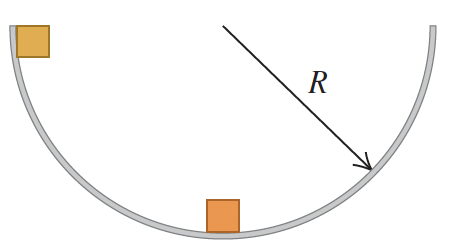
\includegraphics[width=0.5\linewidth]{../figures/P8_82.png}
  \label{fig:P8_82}
\end{figure}

Two identical masses are released from rest in a smooth hemispherical bowl of radius $R$ from the positions shown in (\textbf{\autoref{fig:P8_82}}). Ignore friction between the masses and the surface of the bowl. If the masses stick together when they collide, how high above the bottom of the bowl will they go after colliding?
\bigbreak
I løbet af den første masse, $m_1$'s, fald omdannes al dens potentielle energi til kinetisk energi, idet vi antager at der ikke er nogen friktion. Altså har vi at
 \[
U_{1} = m\cdot g\cdot R
.\] 
Dette omdannes til kinetisk energi så vi har at
\[
m\cdot g\cdot R = \frac{1}{2} \cdot m \cdot \left( v_1 \right)^2  \implies v_1 = \sqrt{2gR} 
.\]
I løbet af stødet antages at der er impulsbevarelse. Altså har vi at
\[
\frac{1}{2} m\cdot v_1^2 = \frac{1}{2} 2m\cdot v_2^2 \implies v_2 = \frac{\sqrt{2}}{2} v_1
.\] 
Den kinetiske energi efter stødet er altså
\[
k_2 = \frac{1}{2} \cdot 2m \cdot \left( \frac{\sqrt{2}}{2} v_1 \right)^2 = \frac{1}{2}m\left( 2gR \right) = m\cdot g\cdot R
.\]
Dette omdannes til potentiel energi så vi får at
\[
  2m\cdot g\cdot h = m \cdot g\cdot R\implies h = \frac{R}{2}
.\] 

\section*{Opg. 8.97}
A fireworks rocket is fired vertically upward. At its maximum height of \qty{80,0}{m}, it explodes and breaks into two pieces: one with mass \qty{1,40}{kg} and the other with mass \qty{0,28}{kg}. In the explosion, \qty{860}{J} of chemical energy is converted to kinetic energy of the two fragments.

\subsection*{(a)}
What is the speed of each fragment just after the explosion?
\bigbreak
Det antages, at de to fragmenter ikke har nogen horisontal komposant til deres hastighed før eksplosionen og at al deres horisontale hastighed derfor er som resultat af eksplosionen. Idet der er impulsbevarelse under eksplosionen har vi derfor at

\begin{equation}
m_1 v_{1_x} + m_2 v_{2_x} = 0
\end{equation}

og at

\begin{equation}
k = \frac{1}{2} \cdot m_1 \cdot \left( v_{1_x} \right)^2 + \frac{1}{2} \cdot m_2 \cdot \left( v_{2_x} \right)^2   
\end{equation}

Vi kan dernæst isolere $v_{2_x}$ i (1) så vi får at

\begin{equation}
v_{2_x} = -\frac{m_1}{m_2}v_{1_x}
\end{equation}

  Dette indsættes i (2) så vi får at
\[
k = \frac{1}{2} \cdot m_1 \cdot \left( v_{1_x} \right)^2 + \frac{1}{2} \cdot m_2 \cdot \left( -\frac{m_1}{m_2}\cdot v_{x_1} \right)^2  = \frac{1}{2}\left( m_1 + \frac{m_1^2}{m_2} \right) v_{1x}^2
.\] 
Vi isolerer dernæst $v_{1_x}$
\[
  v_{1_x} = \sqrt{\frac{2k}{m_1 + \frac{m_1^2}{m_2}}} = \sqrt{\frac{2\cdot \qty{860}{J}}{\qty{1,40}{kg} + \frac{\left( \qty{1,40}{kg} \right)^2}{\qty{0,28}{kg}}}} = \qty{14,31}{\frac{m}{s}} 
.\] 
Dette kan nu indsættes i (3) for at give os $v_{2_x}$ 
\[
v_{2_x} = - \frac{\qty{1,40}{kg}}{\qty{0,28}{kg}}\cdot \qty{14,31}{\frac{m}{s}} = \qty{-69,8}{\frac{m}{s}}
.\] 

\subsection*{(b)}
It is observed that the two fragments hit the ground at the same time. What is the distance between the points on the ground where they land? Assume that the ground is level and air resistance can be ignored.
\bigbreak
Først findes tiden, $t$, brugt på at ramme jorden fra en højde $s_y$ vha. formlen for strækning ved konstant acceleration
\[
  s_y = \frac{1}{2}gt^2 \implies t = \sqrt{\frac{2s_y}{g}} = \sqrt{\frac{2\cdot \qty{80,0}{m}}{\qty{9,81}{\frac{m}{s^2}}}} = \qty{4,04}{s} 
.\] 
Afstanden mellem de to må være givet ved
\[
s_x = (v_{1_x} - (-v_{2_x}))t = \left( \qty{14,31}{\frac{m}{s}} + \qty{69,8}{\frac{m}{s}} \right)\cdot \qty{4,04}{s} = \qty{339,8}{m}
.\] 


\section*{Opg. 8.103}
In a rocket-propulsion problem the mass is variable. Another such problem is a raindrop falling through a cloud of small water droplets. Some of these small droplets adhere to the raindrop, thereby \textit{increasing} its mass as it falls. The force on the raindrop is
\[
F_{ext} = \frac{\mathrm{d}p}{\mathrm{d}t} = m \frac{\mathrm{d}v}{\mathrm{d}t} + v \frac{\mathrm{d}m}{\mathrm{d}t} 
.\]
Suppose the mass of the raindrop depends on the distance $x$ that it has fallen. Then $m = kx$, where $k$ is a constant, and $ \frac{\mathrm{d}m}{\mathrm{d}t} = kv$. This gives, since $F_{ext} = mg$,
\[
mg = m \frac{\mathrm{d}v}{\mathrm{d}t} + v(kv)
.\] 
Or, dividing by $k$,
 \[
xg = x \frac{\mathrm{d}v}{\mathrm{d}t} + v^2
.\] 
This is a differential equation that has a solution of the form $v = at$, where $a$ is the acceleration and is constant. Take the initial velocity of the raindrop to be zero.

\subsection*{(a)}
Using the proposed solution for $v$, find the acceleration $a$.
\bigbreak
Først indses at
\[
v = \frac{\mathrm{d}x}{\mathrm{d}t} 
.\] 
Derudover har vi givet en løsning der er på formen
\[
v = at
.\] 
Altså har vi at
\[
\frac{\mathrm{d}x}{\mathrm{d}t} = at \implies \int \, \mathrm{d}x = \int at \, \mathrm{d}t \implies x = \frac{1}{2}at^2 + x_0
.\] 
Desforuden gælder det at
\[
a = \frac{\mathrm{d}v}{\mathrm{d}t} 
.\] 
Alt dette kan indsættes i differentialligningen så vi får at
\[
  \left( \frac{1}{2}at^2 + x_0 \right)g = \left( \frac{1}{2}at^2 + x_0\right)a + a^2t^2
.\]
Vi sætter $x_0 = 0$ for simplicitetens skyld
 \[
   \left( \frac{1}{2}at^2 \right) g = \left( \frac{1}{2}at^2 \right) a + a^2t^2 = \frac{3}{2}a^2t^2
.\]
Altså har vi
\[
a = \frac{1}{3}g
.\] 

\subsection*{(b)}
Find the distance the raindrop has fallen in $t = \qty{3,00}{s}$ 
\bigbreak
Her benyttes formlen for strækning ved konstant acceleration igen. Altså får vi at
\[
s_y = \frac{1}{2}\cdot \frac{1}{3}\cdot \qty{9,81}{\frac{m}{s^2}}  \cdot \left( \qty{3,00}{s} \right) ^2 = \qty{14,715}{m}
.\] 


\subsection*{(c)}
Given that $k = \qty{2,00}{\frac{g}{m}}$, find the mass of the raindrop
at $t = \qty{3,00}{s}$.
\bigbreak
Vi har at
\[
\frac{\mathrm{d}m}{\mathrm{d}t} = kv = kat = \frac{1}{3}kgt
.\] 
Altså
\[
  \int \, \mathrm{d}m = \frac{1}{3}kgt \, \mathrm{d}t \implies m - m_0 = \frac{1}{6}kgt^2
.\] 
Vi sætter $m_0 = 0$ og får
 \[
m = \frac{1}{6}kgt^2
.\] 
Vi indsætter kendte værdier
\[
m = \frac{1}{6}\cdot \qty{2,00}{\frac{g}{m}} \cdot \qty{9,81}{\frac{m}{s^2}} \cdot \left( \qty{3,00}{s} \right)^2 = \qty{29,43}{g} 
.\] 

\end{document}
